\documentclass[a4paper,12pt]{article}
\usepackage[left = 1.5cm, top = 2cm, right = 1.5cm, bottom = 2cm]{geometry}

\usepackage{graphicx}
\usepackage{booktabs}
\usepackage{caption}
\usepackage{amsmath}
\usepackage{amsfonts}
\usepackage{amsthm}
\usepackage{changepage}
\usepackage{amssymb}
\usepackage{subcaption}
\usepackage{float}
\usepackage[dvipsnames]{xcolor}
\usepackage[most]{tcolorbox}
\usepackage[shortlabels]{enumitem}
\usepackage{pdfpages}
\usepackage{tikz}
\usepackage[numbers,sort&compress]{natbib} % \cite{key}; entries live in references.bib

\usepackage{verbatim}
\usepackage[noend,ruled,linesnumbered]{algorithm2e}
\DontPrintSemicolon
\SetKwInOut{Input}{Input}
\SetKwInOut{Output}{Output}

% Custom commands
\newcommand{\algo}[1]{\emph{\textcolor{blue}{#1}}}
\newcommand{\xor}{\oplus}
\newcommand{\ord}{\text{ord}}
\newcommand{\horiline}{
\noindent\makebox[\linewidth]{
    \rule{\paperwidth}{0.4pt}}
}
\newcommand{\bfhoriline}{
\noindent\makebox[\linewidth]{
    \rule{\paperwidth}{2pt}}
}
\newcommand{\ay}{\mathcal{A}}
\newcommand{\bee}{\mathcal{B}}
\newcommand{\Z}{\mathbb{Z}}
\newcommand{\R}{\mathbb{R}}
\newcommand{\E}[1]{\mathbb{E}\left[ #1 \right]}
\newcommand{\keygen}{\operatorname{KeyGen}}
\newcommand{\enc}{\operatorname{Enc}}
\newcommand{\dec}{\operatorname{Dec}}
\newcommand{\pk}{\operatorname{PK}}
\newcommand{\sk}{\operatorname{SK}}
\newcommand{\green}[1]{\mathcolor{PineGreen}{#1}}
\newcommand{\red}[1]{\mathcolor{red}{#1}}
\newcommand{\blue}[1]{\mathcolor{blue}{#1}}
\newcommand{\mat}[1]{\begin{bmatrix} #1 \end{bmatrix}}
\newcommand{\pmat}[1]{\begin{pmatrix} #1 \end{pmatrix}}
\newcommand{\abs}[1]{\left| #1 \right|}
\newcommand{\norm}[1]{\left\Vert #1 \right\Vert}
\newcommand{\Zmod}[1]{\mathbb{Z}/ #1 \mathbb{Z}}
\newcommand{\Zmodstar}[1]{(\Zmod{ #1 })^*}
\newcommand{\rank}{\operatorname{rank}}
\newcommand{\spank}{\operatorname{span}}
\newcommand{\pderiv}[2]{\frac{\partial #1}{\partial #2}}
\newcommand{\lcm}{\operatorname{lcm}}
\newcommand{\tr}{\operatorname{tr}}

% Custom spacings
\setlength\parindent{0pt}
\setlength{\parskip}{0.75em}

% Custom environemnts
% \begin{lemma} or \begin{lemma}[Case 1: ...] for an underlined heading
\newenvironment{lemma}[1][]
    {\ifstrempty{#1}{}{\underline{#1}\par\nobreak\vspace{0.25em}}%
     \begin{adjustwidth}{1cm}{0cm}}
    {\end{adjustwidth}}



% Beamer-style titled blocks
\definecolor{blocktitle}{RGB}{34,45,120}
\definecolor{blockbody}{RGB}{230,231,243}
\tcbset{blockstyle/.style={
    enhanced, breakable,
    colback=blockbody, colbacktitle=blocktitle, coltitle=white,
    colframe=blocktitle, boxrule=0pt, arc=2pt,
    left=6pt, right=6pt, top=4pt, bottom=4pt,
    fonttitle=\bfseries,
    after skip=1.5em,
    before upper={\setlength{\parskip}{0.6em}}, % restore inter-paragraph gap
}}

% \niceblock[<extra tcolorbox options>]{<title>}{<body>}
%   \niceblock{Theorem 1 (Fermat)}{...}
%   \niceblock[colbacktitle=PineGreen, colframe=PineGreen]{Exercise 2}{...}
\newtcolorbox{niceblockenv}[1][]{blockstyle, #1}
\newcommand{\niceblock}[3][]{%
    \begin{niceblockenv}[title={#2}, #1]%
    #3%
    \end{niceblockenv}%
}

% Same block without a title bar, and for bodies that \niceblock cannot take as
% an argument (verbatim, \begin{comment}, ...):
%   \begin{niceblockenv}[title={Theorem 1}] ... \end{niceblockenv}

% Numbered, cross-referenceable blocks. All kinds share one counter, so numbers
% are unique: Definition 1.1, Theorem 1.2, Exercise 1.3, ... (reset each section).
\newcounter{niceblockcounter}

% \newniceblock{<cmd>}{<Heading>}{<extra tcolorbox options>}
%   defines \<cmd>[<options>]{<name>}{<body>} and the environment <cmd>env
\newcommand{\newniceblock}[3]{%
    \newtcolorbox[use counter=niceblockcounter, number within=section]{#1env}[2][]{%
        blockstyle,
        title={#2~\thetcbcounter\ifstrempty{##2}{}{: ##2}},
        #3, ##1%
    }%
    \expandafter\newcommand\csname #1\endcsname[3][]{%
        \begin{#1env}[##1]{##2}##3\end{#1env}%
    }%
}

% Usage: \definition[label=def:shannon]{Shannon Entropy}{...} -> "Definition 1.1: Shannon Entropy"
%        \theorem{}{...}                                      -> "Theorem 1.2" (no name)
% then refer to it anywhere with \ref{def:shannon}.
% NOTE: \newniceblock{lemma}{Lemma} would clash with the lemma environment above.
\newniceblock{definition}{Definition}{}
\newniceblock{theorem}{Theorem}{}
\newniceblock{exercise}{Exercise}{colbacktitle=PineGreen, colframe=PineGreen,
    segmentation style={solid, PineGreen, line width=0.6pt}}

% Message arrows for two-party game diagrams (challenger / adversary).
% The \makebox sets a minimum arrow length so short labels still look right.
\newcommand{\msgto}[1]{\xrightarrow{\makebox[2.2cm]{$\scriptstyle #1$}}}
\newcommand{\msgfrom}[1]{\xleftarrow{\makebox[2.2cm]{$\scriptstyle #1$}}}

% Styles for the Alice--Bob--Eve channel diagrams. Parties reuse the block
% colours; anything belonging to the adversary is red.
\usetikzlibrary{arrows.meta, positioning, calc, fit, backgrounds}
\tikzset{
    party/.style={draw=blocktitle, fill=blockbody, rounded corners=2pt,
        line width=0.8pt, inner sep=6pt, font=\bfseries, minimum width=1.5cm},
    adversary/.style={party, draw=red!65!black, fill=red!8},
    blackbox/.style={draw=red!65!black, fill=red!8, rounded corners=2pt,
        line width=0.8pt, inner sep=6pt, minimum width=1.5cm},
    wire/.style={-{Stealth[length=2.2mm]}, line width=0.8pt},
    leak/.style={wire, densely dashed, red!65!black},
    wirelab/.style={font=\small, inner sep=2pt},
    note/.style={font=\scriptsize\itshape, inner sep=2pt},
    region/.style={draw=red!65!black, densely dotted, rounded corners=4pt,
        inner sep=10pt, line width=0.7pt},
}

%============================================%
%============= Useful Structures ============%
%============================================%

%====== Table %======%

% \begin{table}[H]
%     \centering
%     \caption{--}
%     \label{tab:my_table}
%     \begin{tabular}{@{} l c c @{}}
%         \toprule
%         \textbf{--} & \textbf{--} & \textbf{--} \\
%         \midrule
%         -- & -- & -- \\
%         -- & -- & -- \\
%         -- & -- & -- \\
%         \bottomrule
%     \end{tabular}
% \end{table}

%====== Figure %======%

% \begin{figure}[H]
%     \centering
%     \includegraphics[width=0.6\linewidth]{figure.png}
%     \caption{--}
%     \label{fig:my_figure}
% \end{figure}

%====== a,b,c enumerate %======%

% \begin{enumerate}[a)]
%     \item First part
%     \item Second part
% \end{enumerate}


\usepackage{hyperref} % hyperref package (should be loaded last)

\hypersetup{breaklinks=true,colorlinks,linkcolor=blue,urlcolor=blue,pdfpagemode=UseNone}

\begin{document}

\title{A BIT About Entropy}


\section{Introduction}

``Entropy'' is a very overloaded term with a range of different meanings across and within different domains of math and science.


\begin{figure}[H]
    \centering
    \begin{subfigure}[b]{0.36\linewidth}
        \centering
        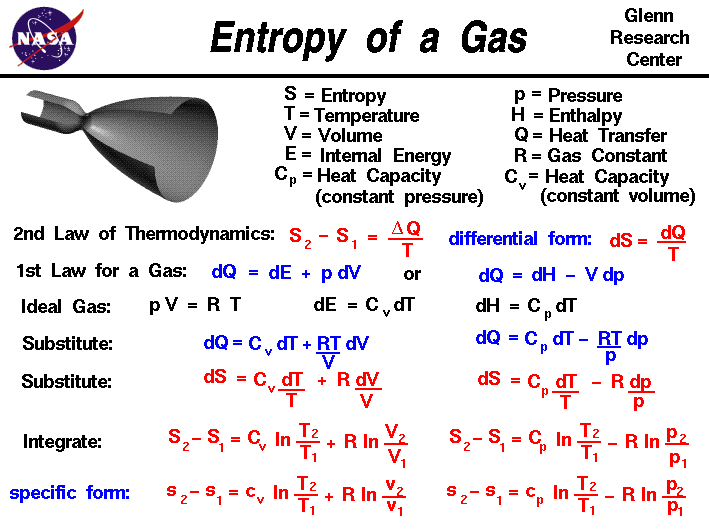
\includegraphics[height=4.5cm]{images/therodynamic_entropy.png}
        \caption{Thermodynamic entropy of a gas \cite{nasa_entropy}}
        \label{fig:thermodynamic_entropy}
    \end{subfigure}
    \hfill
    \begin{subfigure}[b]{0.33\linewidth}
        \centering
        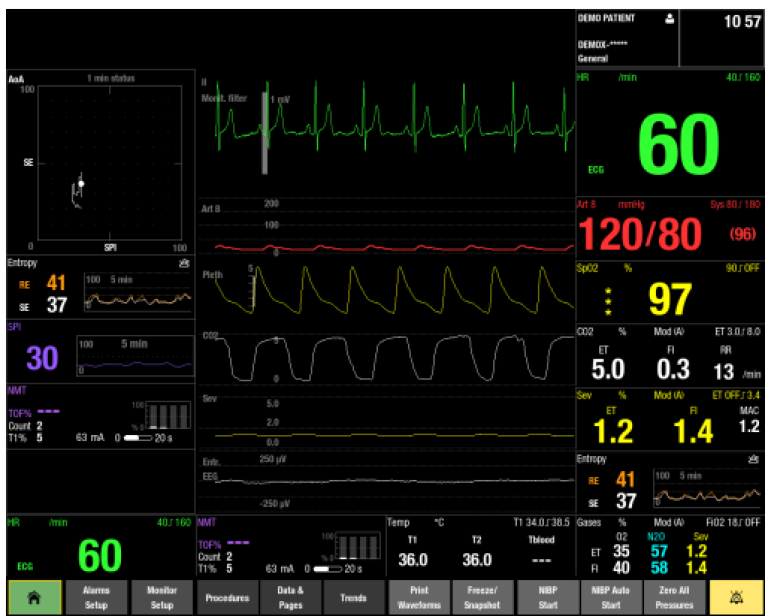
\includegraphics[height=4.5cm]{images/eeg_entropy.png}
        \caption{EEG entropy on a patient monitor \cite{ge_entropy_monitoring}}
        \label{fig:eeg_entropy}
    \end{subfigure}
    \hfill
    \begin{subfigure}[b]{0.22\linewidth}
        \centering
        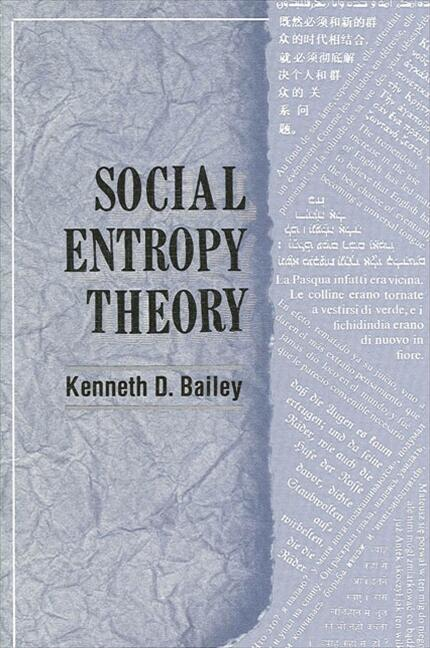
\includegraphics[height=4.5cm]{images/social_entropy.jpg}
        \caption{Social entropy \cite{bailey1990}}
        \label{fig:social_entropy}
    \end{subfigure}
    \caption{A few of the many things called ``entropy''.}
    \label{fig:entropies}
\end{figure}

The link between many of these is more spiritual than anything else: entropies ``quantify uncertainty and information''.
Today, we'll focus on entropy in the context of information theory.
That is, how can we mathematically model uncertainty and the transfer of information?

\section{Shannon entropy}

Let's start with an exercise from \cite{nielsen2010} that describes pretty well how the mathematical formula for entropy was discovered.
Starting with the desired properties, we can derive a derive that entropy should take a given form:

\begin{figure}[H]
    \centering
    % Two halves of one exercise; widths keep the scanned text at the same size.
    \begin{minipage}{0.8\linewidth}
        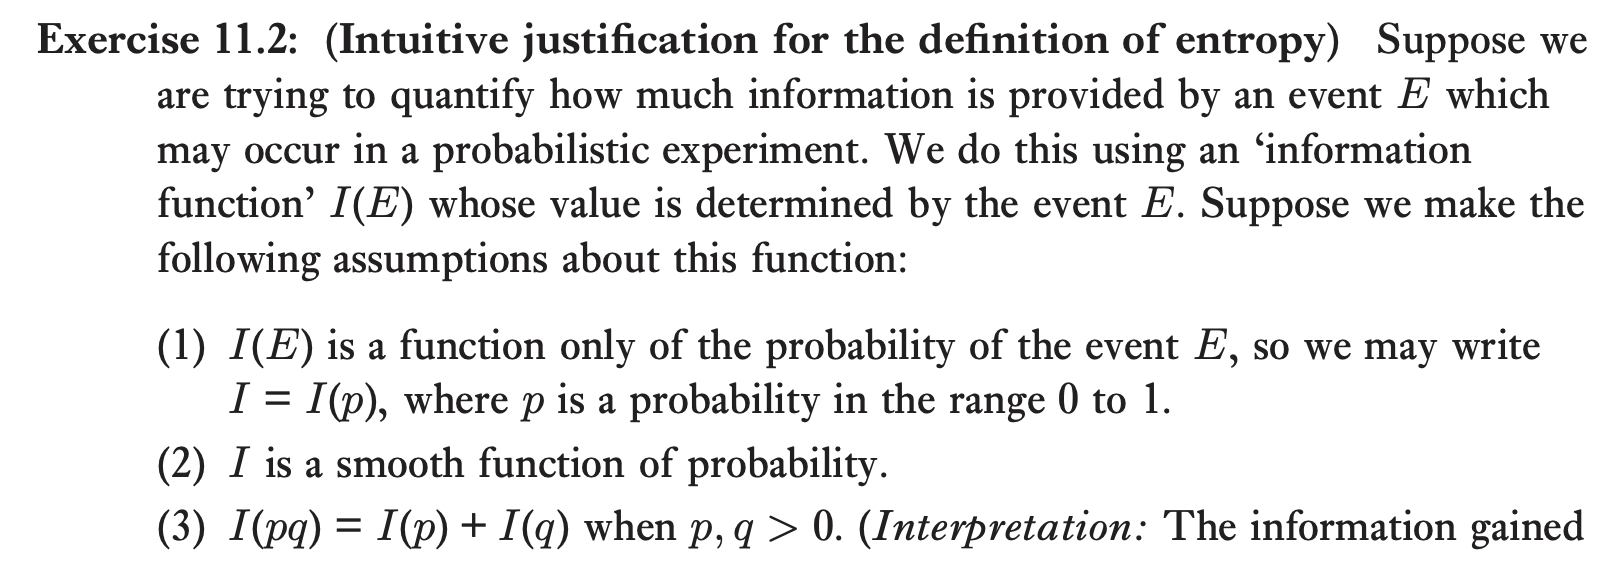
\includegraphics[width=\linewidth]{images/exercise_1.png}\\
        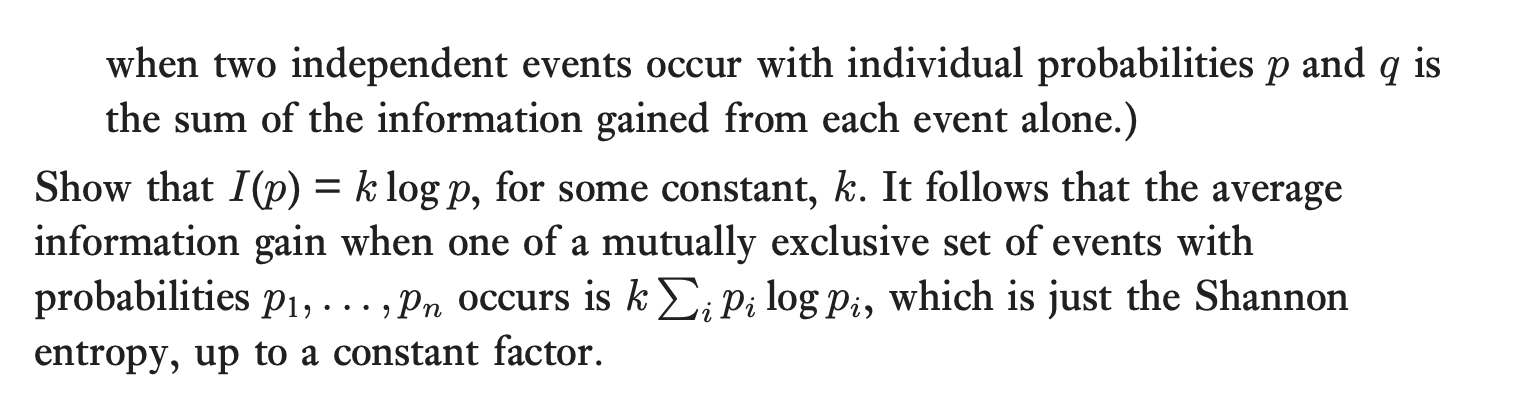
\includegraphics[width=0.938\linewidth]{images/exercies_2.png}
    \end{minipage}
    \caption{Exercise 11.2 from \cite{nielsen2010}.}
    \label{fig:exercise_entropy}
\end{figure}


This is similar to how Claude Shannon invented Shannon entropy in his seminal 1948 paper ``A Mathematical Theory of Communication'' \cite{shannon1948}.
We define Shannon entropy as follows:

\definition[label=def:shannon]{Shannon entropy}{
    For a discrete, random variable $X=1,...,n$ with probability distribution $p_1,...,p_n$, the Shannon entropy is defined as:
    $$H(X) \equiv H(p_1, ..., p_n)\equiv-\sum_x p_x \log p_x$$
}
There are two parts of this formulation which are particularly ambigious.

First, we need to make the exception that if $p_x=0$, then we neglect the term by agreeing $0\log 0 \equiv 0$.
Intuitively, if $p_x=0$, then $X$ can never take the value of $x$, so why should this case affect the entropy!

Second, what is the base of the logarithm?
We will see later that taking logarithms in base 2 allows for a meaningful connection to the number of bits needed to represent data pertaining to $X$ in binary.
This is part of the reason why bits is said to be the unit for $H(X)$.
That is, we say $X$ has $H(X)$ \emph{bits of entropy}.

Something else to notice is that the entropy $H(X)$ does not depend on the labels of what $X$ can take, and is only a function of its distribution.

Let's play with this a little bit to get a feel for the formula:
\exercise{Playing with Shannon entropy}{
    \begin{enumerate}
        \item What is the entropy associated with the toss a fair coin?
        \item What is the entropy associated with the roll of a fair die?
        \item What is the entropy associated with the roll of a \emph{Mario die} (with sides 1,3,3,3,5,6)? What about a \emph{Peach die} (0,2,4,4,4,6)?
        \item How do the above compare to a fair 4-sided die?
    \end{enumerate}
}

So we understand how to calculate Shannon entropy, but what is the intuition behind it representing a quantity of information?
One answer is that it captures \emph{the physical resources needed to communicate information}.

Suppose we have an information source, which is constantly producing i.i.d. discrete random variables $X_1,X_2,...$.
What is the expected amount of minimal physical ressources we need to send, on average, so that this string of random variables can be perfectly reconstructed by the receiver?
The answer, amazingly, is $H(X)=H(X_1)=H(X_2)...$ bits!

Let's consider a simple example (from \cite{nielsen2010}). 
Consider a source of information that produces a sequence of four signals: $X=A, B, C,\text{ or } D$.
Now suppose that the sources wanted to send this sequence to some receiver by encoding the symbols into binary.
We know that we can build an encoding scheme that uses 2 bits to represent each symbol:

\begin{table}[H]
    \centering
    \begin{tabular}{@{} l c c c c @{}}
        \toprule
        \textbf{Symbol} & $A$ & $B$ & $C$ & $D$ \\
        \midrule
        \textbf{Encoding} & \texttt{00} & \texttt{01} & \texttt{10} & \texttt{11} \\
        \bottomrule
    \end{tabular}
\end{table}

But now suppose we know that these symbols aren't generated uniformly, and that we know the distribution:

\begin{table}[H]
    \centering
    \begin{tabular}{@{} l c c c c @{}}
        \toprule
        \textbf{Symbol} & $A$ & $B$ & $C$ & $D$ \\
        \midrule
        \textbf{Probability} & $1/2$ & $1/4$ & $1/8$ & $1/8$ \\
        \bottomrule
    \end{tabular}
\end{table}

Then we can come up with an encoding scheme that leverages this:

\begin{table}[H]
    \centering
    \begin{tabular}{@{} l c c c c @{}}
        \toprule
        \textbf{Symbol} & $A$ & $B$ & $C$ & $D$ \\
        \midrule
        \textbf{Probability} & $1/2$ & $1/4$ & $1/8$ & $1/8$ \\
        \textbf{Encoding} & \texttt{1} & \texttt{10} & \texttt{110} & \texttt{111} \\
        \bottomrule
    \end{tabular}
\end{table}

This scheme yeilds an expected number of bits per symbol to be

$$ 1\left(\frac{1}{2}\right) + 2\left(\frac{1}{4}\right) + 3\left(\frac{1}{8}\right) + 3\left(\frac{1}{8}\right) = \frac{7}{4}. $$

Sure enough, if we calculate the entropy of the distribution of symbols:

\begin{flalign*}
    -\frac{1}{2}\log\left(\frac{1}{2}\right) - \frac{1}{4}\log\left(\frac{1}{4}\right) - \frac{1}{8}\log\left(\frac{1}{8}\right) - \frac{1}{8}\log\left(\frac{1}{8}\right) \\
    = \frac{1}{2}\cdot 2 + \frac{1}{4}\cdot 2 + \frac{1}{8}\cdot 3 + \frac{1}{8}\cdot 3 \\
    = \frac{7}{4}
\end{flalign*}

So this isn't just a good encoding scheme, its the best we can possibly do!

Lets give a quick, semi-formal proof of this optimality (following from \cite{duplantier2021}).
Suppose that we want to transmit some large, but finie sequence of $N$ symbols $X=1,2,...,m$ drawn i.i.d. with probabilities $P(X=i)=p(i)$.
Because each symbol is drawn i.i.d, the probability of getting any one sequence $\bar{x}=(x_1,...,x_N)$ is
$$p(\bar{x}) = p(x_1)p(x_2)\cdots p(x_N)$$
We can collect terms which have the same symbol, where $n(i)$ is the number of symbols in $\bar{x}$ which are $i$:
$$p(\bar{x}) = \prod_{i=1}^m p(i)^{n(i)}$$
By the law of large numbers, we know that as $N\to \infty$, we can use the probability of each symbol in order to estimate $n(i) \approx Np(i)\cdot$, giving us:
$$p(\bar{x})\approx \prod_{i=1}^m p(i)^{Np(i)} = \prod_{i=1}^m \left(2^{\log p(i)}\right)^{Np(i)}  = 2^{-NH(X)}$$

So if $n(i)=Np(i)$, then the probability of getting this sequence becomes $2^{-NH(X)}$.
If $N$ is large enough, we can safetly ignore sequences that don't satisfy $n(i)=Np(i)$ to arbitrary precision, since that becoms exponentially more unlikely.
We call the sequences that satisfy this \emph{typical sequences}.
Suppose that leaves us with $M$ such typical sequences left after excluding the \emph{atypical} ones.
Summing over $p(\bar{x})=2^{-NH(X)}$ yeilds $1\approx M2^{-NH(X)}$.
So there are (approximately $M\approx2^{NH(X)}$) typical sequences.
If we index these, we can therefore send $\log M$ bits to communicate which typical sequence we are trying to send.



\section{Entropy as a Measure of Security}

Suppose you had a random variable $X=1,...,n$.
After $X$ is drawn at random, suppose you can ask yes or no questions of the form ``is $X$ in the subset $S\subset\{1,...,n\}$?''
How many guesses, on average, will it take you to be able to figure out the value of $X$?

The answer, as it turns out, is $2^{H(X)}$! The proof of this is left as homework (\emph{hint: how does prefix-free encoding relate to binary trees?}).

Now, imagine that $X$ is a random user's password.
We can use entropy as a measure of the uncertainty an attacked might have about this password.
Despite the fact that a user \emph{is allowed} to have their password be consist of 20-30 random characters, the \emph{real} distribution of passwords in practice is quite skewed.

\begin{figure}[H]
    \centering
    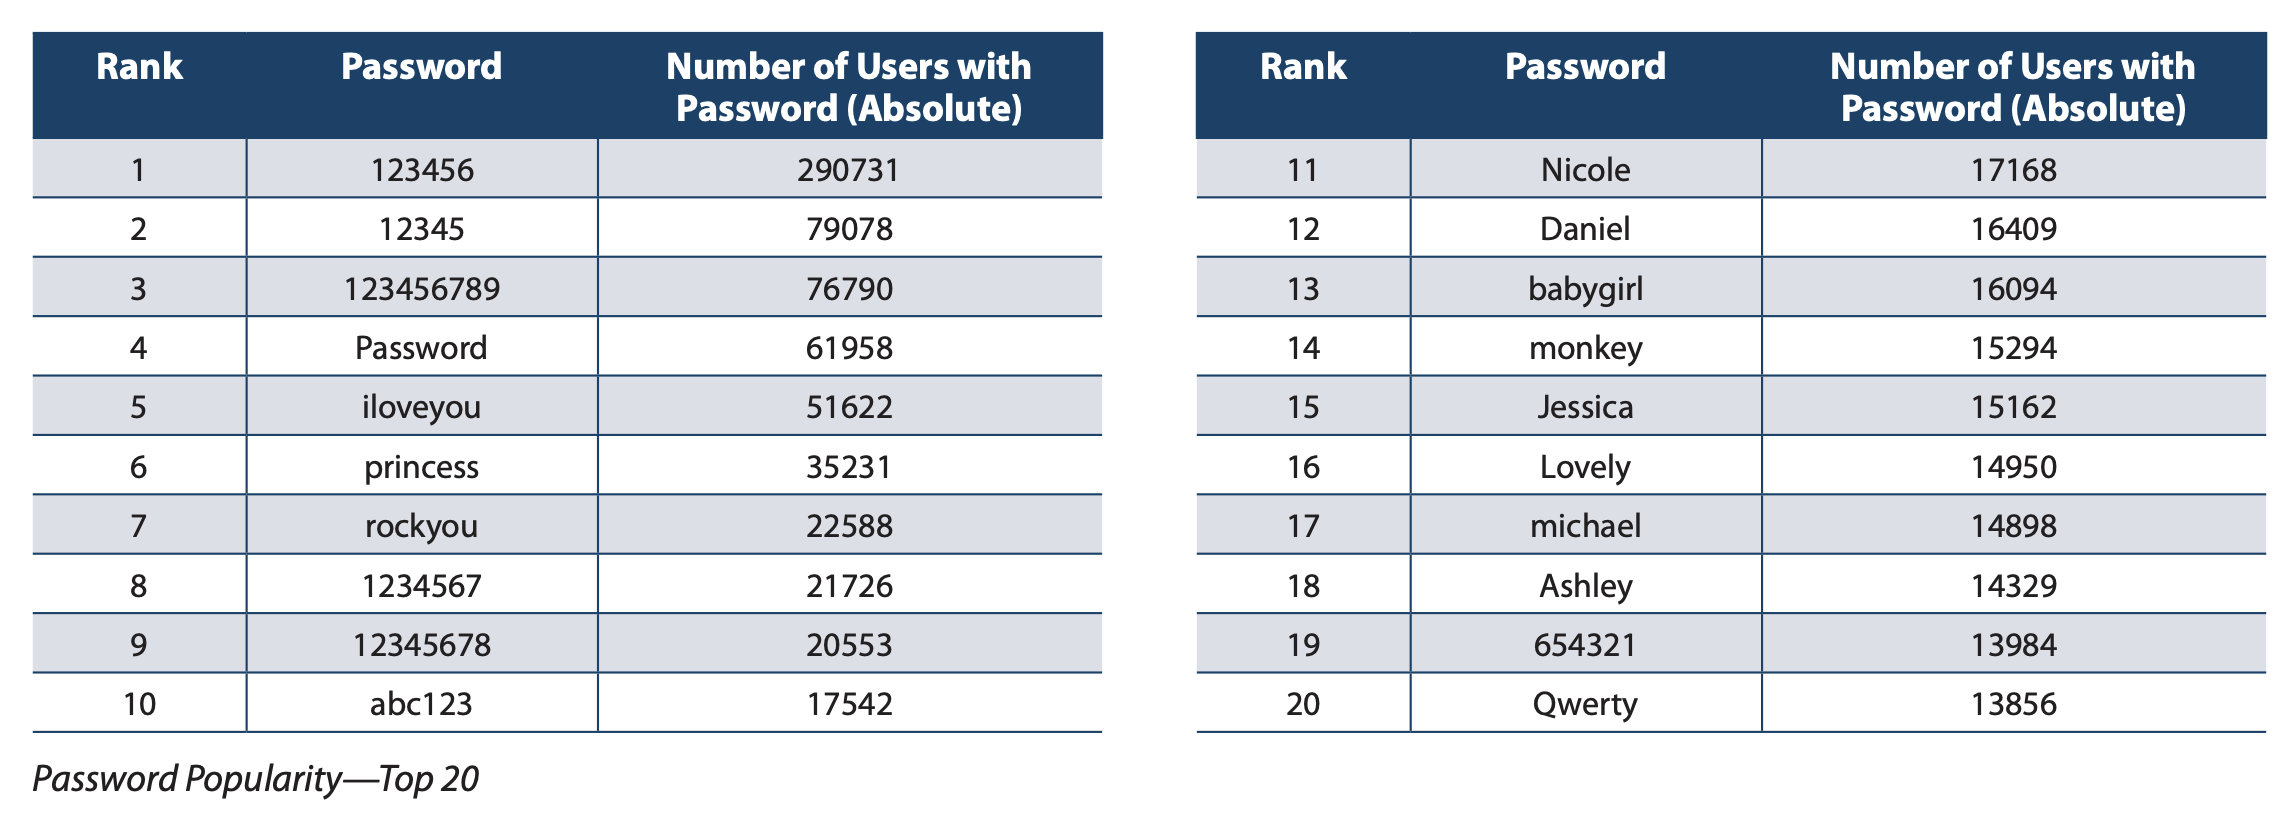
\includegraphics[width=0.9\linewidth]{images/rock_you.png}
    \caption{The 20 most common passwords among the 32 million leaked in the 2009 RockYou breach \cite{imperva2010}.}
    \label{fig:rock_you}
\end{figure}
The Shannon entropy of the full RockYou password distribution has been estimated at only about $21.15$ bits \cite{bonneau2012}.

The additive property of entropy also tells us how to build more secure passwords: we can simply append more randomness to the end.

There are a couple limitations to this line of reasoning though.

First, is that there is a misalignement between our previous guesswork model and how guessing passwords is a actually done.
Analysis on real password databases has shown that the Shannon entropy does not correlate with difficulty when passwords need to be guessed one-at-a-time \cite[p.~44]{bonneau2012thesis}.

% Quote: "For an attacker who must guess possible values individually, Shannon entropy has no direct correlation to guessing difficulty."

Second, is that real password attacks don't take this shape.
Let's look at a failure case.

Imagine our userbase is distributed as follows: half the users are secure, and pick a random password from a pool of $2^{128}$, and the other half are lazy, and just pick the word ``password'' as their password.
So $X=\text{``password''}$ with probability $\frac{1}{2}$, and each of the $2^{128}$ random passwords shows up with probability $\frac{1}{2}\cdot 2^{-128} = 2^{-129}$.
The entropy of this password distribution is:
$$H(X) = -\underbrace{\frac{1}{2}\log\frac{1}{2}}_{\text{half the users using ``password''}} - \underbrace{2^{128}\cdot 2^{-129}\log 2^{-129}}_{\text{half the users picking at random}} = \frac{1}{2} + \frac{129}{2} = 65 \text{ bits}$$

This seems pretty secure! 65 bits is the same uncertainty as a password chosen uniformly from $2^{65}$ possibilities, which would take an attacker an huge amount of guessing.
But for half the users, an attacker can guess the password as ``password'' on the very first try. If this doesn't work... they can simply pick another user to attack.

The problem is that $H(X)$ averages over the whole distribution, so the enormous uncertainty of the secure half drowns out the fact that the lazy half have no uncertainty at all.
An attacker doesn't care about the average; they care about their best guess.
This is captured by the \emph{min-entropy}:
$$H_\infty(X) = -\log \max_x p(x) = -\log\frac{1}{2} = 1 \text{ bit}$$
From the attacker's point of view, this userbase is about as secure as a coin flip.
Notice also that we can make $H(X)$ as large as we like by growing the pool the secure users pick from, without changing $H_\infty(X)$ at all: the weakest passwords stay exactly as weak.
For this reason, min-entropy is the measure NIST uses when assessing the entropy sources that feed cryptographic random number generators \cite{nist80090b}.

\section{Acknowledgements}

\begin{enumerate}
    \item CO487 Course notes
    \item Claude for aiding with latex typsetting
\end{enumerate}

\bibliographystyle{unsrtnat}
\bibliography{references}

\end{document}



